\documentclass[11pt,a4paper]{article}
\usepackage[margin=23mm]{geometry}
\usepackage[T1]{fontenc}
\usepackage{lmodern}
\usepackage{amsmath,amssymb}
\usepackage{graphicx,placeins,booktabs}

\begin{document}
\noindent\textbf{Working section draft.} This document is separate from the main
manuscript. It records the comparison rationale and agreed scope. The expanded
validation and timing protocol below is proposed work, not completed evidence.

\section{Comparison with model predictive control}
\label{sec:mpc-comparison-draft}

The comparison assesses the performance and online computation of conditioned
proportional switching-time feedback relative to model predictive control
(MPC). The proportional controller uses a fixed gain designed offline and a
solver-free dwell-time conditioner. MPC optimizes a sequence of admissible
timing actions online and applies its first action. The question is how much
performance is lost by restricting the applied action to the direction of the
proportional request, and how much computation this restriction saves.

MPC optimality concerns its specified constrained prediction problem. It does
not imply that every closed-loop performance measure improves on the exact
plant. Stability must also be assessed separately from performance. The
common quadratic certificate for conditioned proportional feedback concerns
the linearized cycle model. MPC's terminal ingredients support a nominal
prediction-model stability argument whose assumptions must be checked. Neither
argument alone certifies the full large-error nonlinear transient.

\subsection{Shared control problem}

All controllers use the same converter benchmark, reference periodic trajectory,
fixed nine-interval mode sequence, and cycle anchor. Only the eight interior
switching instants move. The cycle period is $286\,\mu\mathrm{s}$ and every
applied dwell duration must be at least $3\,\mu\mathrm{s}$. These are the
existing study settings; the dwell bound is not a hardware-calibrated limit.

Let $e_k$ denote the physical cycle-start error. The normalized state and
applied timing input are
\[
    z_k=S_x^{-1}e_k,\qquad
    v_k=\frac{\delta\tau_k^{\mathrm{app}}}{t_s},\qquad
    S_x=\operatorname{diag}(10,20,1),\quad t_s=10\,\mu\mathrm{s}.
\]
The common linearized prediction model is $z_{k+1}=Az_k+Bv_k$.
The conditioned proportional law applies
\[
    v_k=-\beta_k K_n z_k,\qquad 0<\beta_k\leq 1,
\]
where $K_n$ is the fixed aggressive LQR gain and $\beta_k$ is the largest
feasible common scale satisfying all dwell constraints. It maximizes this
scale along the requested direction, not a constrained tracking objective.

The MPC comparator optimizes all eight input components in each predicted
cycle with a five-cycle horizon, $H=5$, and is denoted MPC-5. Its cost is equivalent to
\[
    \sum_{j=0}^{H-1}
    \left(z_{j|k}^{\mathsf T}Qz_{j|k}
    +v_{j|k}^{\mathsf T}Rv_{j|k}\right)
    +z_{H|k}^{\mathsf T}P_f z_{H|k},
    \qquad Q=I_3,\quad R=0.001 I_8.
\]
Here $P_f$ is the LQR Riccati terminal weight. The prediction also imposes
an invariant terminal set under the corresponding raw LQR law. The native
implementation rescales the whole objective without changing its optimizer.
All controllers update once per cycle. As a consistency check, inactive-constraint
MPC must recover the same raw LQR action; this check already exists in the study.

\subsection{Evaluation criteria}

The primary performance measure is the accumulated tracking-and-timing cost
\begin{equation}
    J_{\mathrm{eval}}=
    \sum_{k=0}^{M-1}
    \left(z_k^{\mathsf T}Qz_k+v_k^{\mathsf T}Rv_k\right),
    \qquad M=100.
    \label{eq:mpc-comparison-evaluation-cost}
\end{equation}
This cost uses the simulated states and applied timing inputs over the same
evaluation window for every controller. It is not the optimized prediction
cost, and it includes no terminal penalty. The evaluation length $M$ is
distinct from the MPC prediction horizon $H$.

Secondary measures are sustained threshold crossing, peak physical-state
excursions, minimum applied dwell, solver failures, and computation time.
Threshold crossing requires $\|z_k\|_2<0.01$ at every remaining simulated
cycle boundary. It is a finite-run observation, not a stability proof.
Incomplete trials have no full-window cost and must be reported as failures,
not silently omitted. Success rates and costs among completed trials must be
reported together.

Figure~\ref{fig:mpc-error-cost} shows how error decays and cost accumulates
over elapsed time, rather than reducing each response to a single bar.
MPC-5 crosses the error threshold earlier than LQR-Daniel at each initial-error
scale. Its accumulated cost is also lower, and the curves reveal when that
difference arises during the transient. The circles identify the first sustained
threshold crossings. These three scales follow only one initial-error direction.

\begin{figure}[htbp]
    \centering
    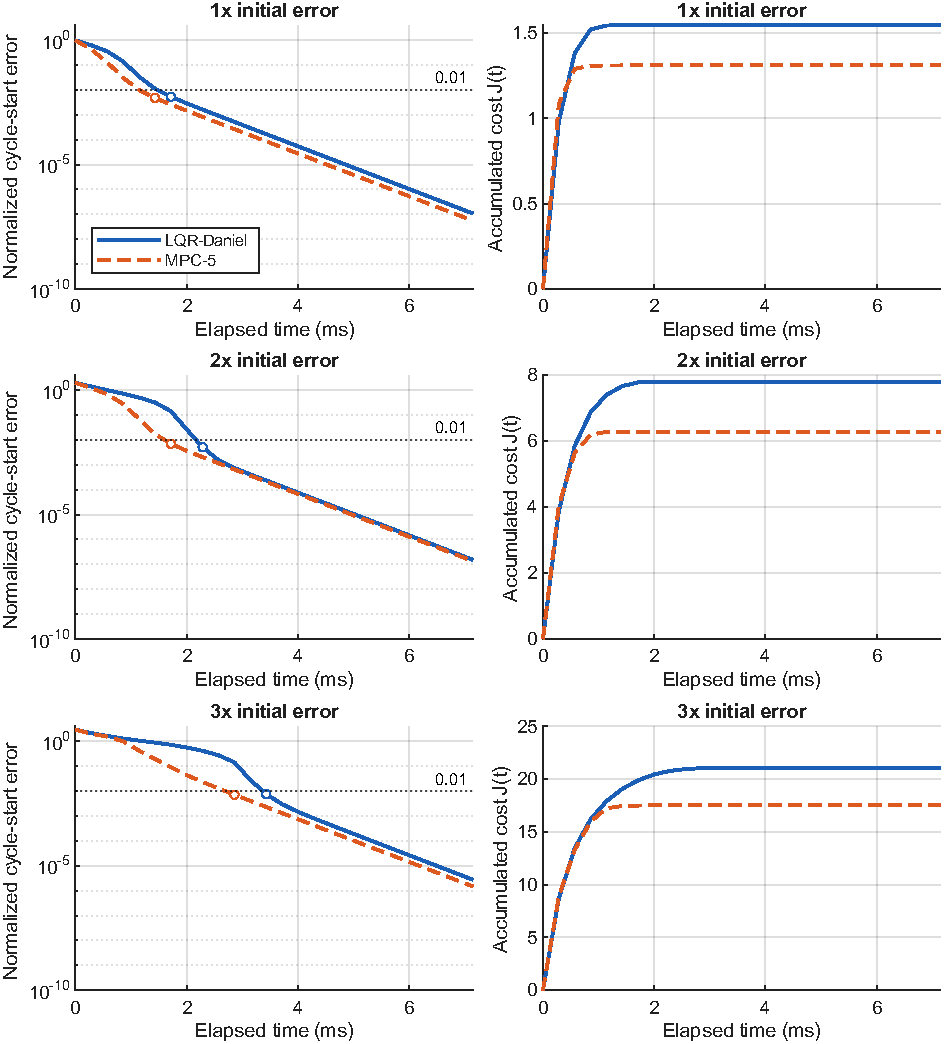
\includegraphics[width=\linewidth]{results/article-figures/error-cost-histories.pdf}
    \caption{Error and accumulated tracking-and-timing cost over the first
    25 nominal periods at $1\times$, $2\times$, and $3\times$ initial error.
    Circles mark sustained error-threshold crossings. Full evaluation costs
    retain the 100-cycle window.}
    \label{fig:mpc-error-cost}
\end{figure}
\FloatBarrier

\subsection{Preliminary trajectory comparison}

Figure~\ref{fig:mpc-conditioning} aligns the $3\times$ error history with
conditioning activity and dwell feasibility. The raw proportional request
initially produces a negative minimum dwell and is not executable. Scaling the
complete request keeps its applied dwell at or above the bound. As the error
falls, the conditioning factor reaches one and the full raw action becomes
admissible in this trial. MPC-5 satisfies the same applied dwell bound through
its optimization constraints; it has no corresponding conditioning factor.

\begin{figure}[htbp]
    \centering
    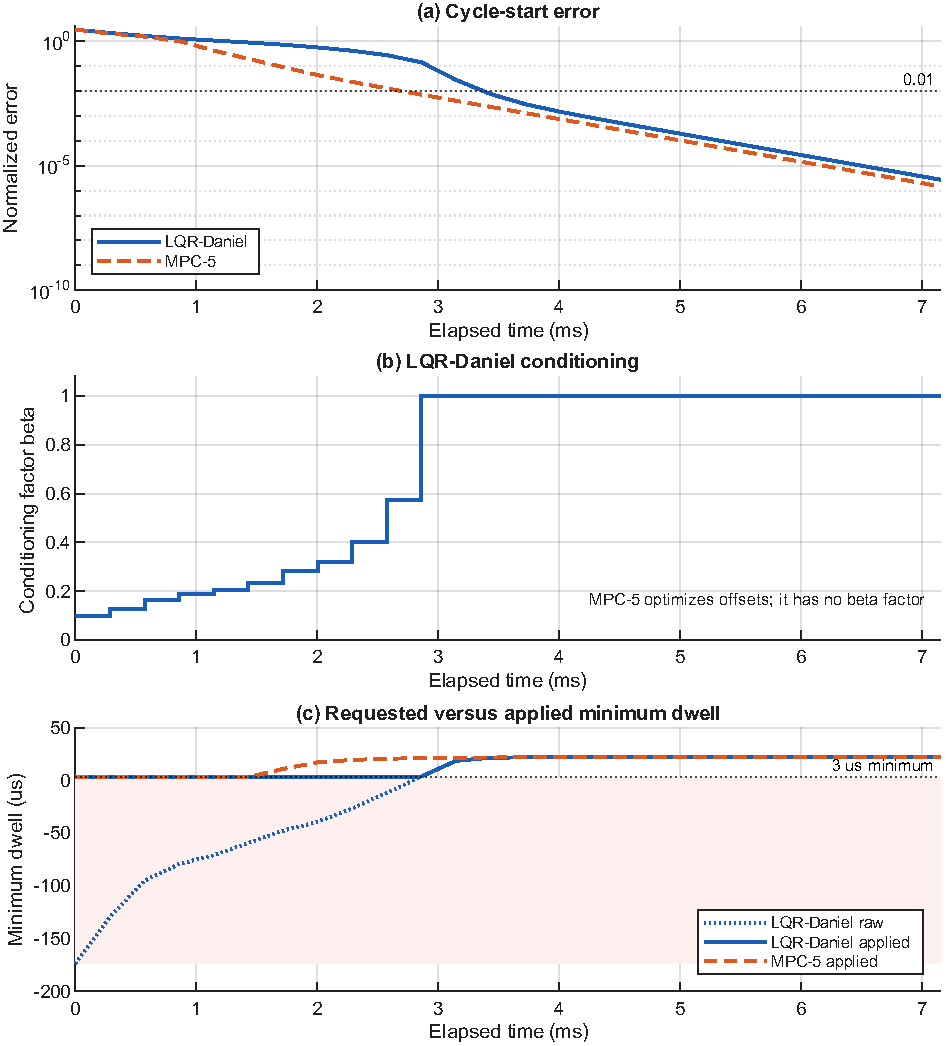
\includegraphics[width=\linewidth]{results/article-figures/conditioning-3x.pdf}
    \caption{Aligned $3\times$ histories over the first 25 periods. Top:
    cycle-start error. Middle: Daniel's conditioning factor. Bottom: raw and
    applied minimum dwells; the shaded region violates the applied bound.
    Dwell and conditioning values belong to the schedule requested at each
    plotted cycle start.}
    \label{fig:mpc-conditioning}
\end{figure}
\FloatBarrier

Earlier threshold crossing does not imply smaller physical excursions.
Figure~\ref{fig:mpc-physical-states} shows MPC-5 driving the first capacitor
voltage below zero before approaching the reference periodic waveform. The
trial also starts with negative current. Neither controller currently constrains
these physical states, so these observations require an
explicit operating envelope before a hardware interpretation is made. The
reference is the time-varying periodic trajectory, not the cycle anchor or an
average operating point.

\begin{figure}[htbp]
    \centering
    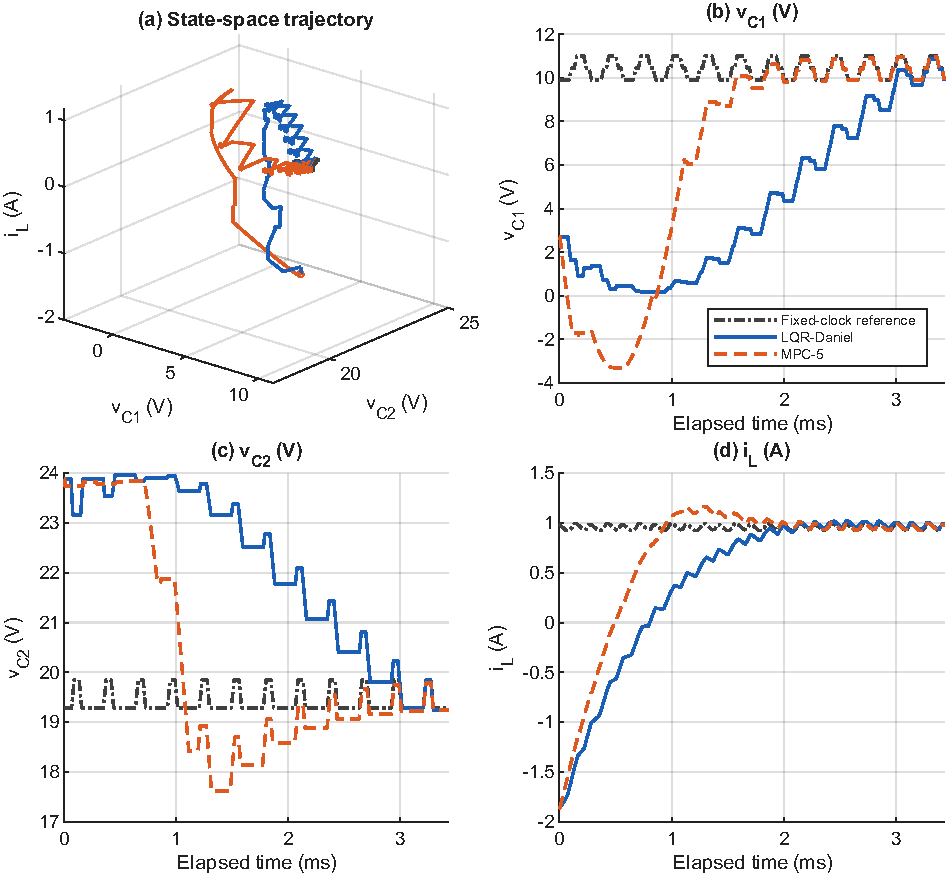
\includegraphics[width=\linewidth]{results/article-figures/physical-trajectories-3x.pdf}
    \caption{State-space paths and physical states over the same twelve-period
    window at $3\times$. The gray reference retains switching ripple.
    Each trajectory uses its own saved sample times. MPC-5 produces a negative
    first-capacitor voltage.}
    \label{fig:mpc-physical-states}
\end{figure}
\FloatBarrier

These figures describe simulated behavior. They do not prove nonlinear
stability or recursive feasibility of the exact controlled plant.

\subsection{Staged validation protocol}

The first phase isolates the nominal-model tradeoff before introducing
uncertainty or hardware effects.
\begin{enumerate}
    \item Evaluate all controllers on the linearized cycle model. Check the
    proportional controller's common quadratic certificate and the assumptions
    behind MPC's terminal-set invariance, recursive feasibility, and nominal
    stability argument. Record optimization feasibility and numerical residuals.
    \item Repeat the same initial conditions with exact switched-affine
    propagation. Retain the same controller models, weights, constraints, and
    evaluation window. Compare costs, state excursions, and one-cycle prediction
    errors to identify changes associated with model mismatch.
\end{enumerate}
The existing $1\times$, $2\times$, and $3\times$ initial-error trials follow
one direction only. Expanded coverage should include different normalized
error directions, inactive and active dwell constraints, and states near the
MPC feasible-region boundary. The initial-condition set and sampling rule must
be specified before running this expanded comparison.

The physically admissible voltage and current envelope remains to be defined.
The existing scaled trials are mathematical stress tests, not validated
hardware operating conditions. Physical state limits are not currently
constraints of any controller. Disturbances, parameter uncertainty,
measurement noise, and computation delays belong to a later phase.

\subsection{Online computation}

Table~\ref{tab:mpc-summary} retains scalar performance and computation
summaries without using a separate sparse timing chart. MPC-5 has lower
100-cycle cost and earlier sustained threshold crossing than LQR-Daniel, but
higher recorded median and p95 host computation time at every tested scale.
These are single ordered host runs, not a controlled timing benchmark.
The time-resolved figures show the response behind the scalar performance values.

\begin{table}[htbp]
    \centering
    \small
    \begin{tabular}{llrrrr}
\toprule
Scale & Method & $J_{\mathrm{eval}}$ & $t_{0.01}$ (ms) & Median ($\mu$s) & p95 ($\mu$s) \\ \midrule
1x & LQR-Daniel & 1.5456 & 1.716 & 12.70 & 145.15 \\ 
1x & MPC-5 & 1.3099 & 1.430 & 265.75 & 2200.20 \\ 
2x & LQR-Daniel & 7.8071 & 2.288 & 12.20 & 17.05 \\ 
2x & MPC-5 & 6.2892 & 1.716 & 262.20 & 688.90 \\ 
3x & LQR-Daniel & 21.074 & 3.432 & 9.35 & 18.05 \\ 
3x & MPC-5 & 17.521 & 2.860 & 301.40 & 972.15 \\ 
\bottomrule
\end{tabular}

    \caption{Saved 100-cycle costs, sustained threshold times, and host timings.
    Timings include first-call overhead. Daniel times feedback and conditioning;
    MPC-5 times its QP solve.}
    \label{tab:mpc-summary}
\end{table}
\FloatBarrier

A matched timing experiment should measure the complete state-to-schedule
computation for both controllers, excluding plant propagation and offline
design. It should separate first-call overhead from warmed execution, include
a shifted-plan warm-start variant for MPC, and report median, p95, p99, and
observed maximum times. Repeated measurements at shared state inputs can
separate implementation cost from differences in the trajectories visited.
Timing along each controller's own trajectories should also be retained.
Desktop measurements do not establish embedded deadlines or worst-case
execution times.

The saved timing measurements include first-call overhead and do not use a
shifted-plan warm start. They also time slightly different portions of the
control paths. They are preliminary evidence of a tradeoff between performance and
computation, not the final matched benchmark. Numerical tables remain owned by
the study's saved results and should be generated from those outputs when the
expanded evidence is ready for publication.
\end{document}
